\lab{Вынужденные колебания в электрическом контуре}

\aim{исследование вынужденных колебаний и процессов их
установления в колебательном контуре.}

\equip{генератор звуковых частот, вольтметр, частотомер, конденсатор, 
    катушка индуктивности, магазин сопротивлений, осциллограф, 
    универсальный измеритель импеданса ($LCR$-метр).}

Перед выполнением работы следует ознакомиться с теоретическим введением
к разделу (п. \ref{sec:forced}--\ref{sec:ust}).

В работе исследуются колебания, возникающие в параллельном электрическом 
контуре под действием внешней ЭДС, гармонически меняющейся во времени.

При подключении к контуру внешнего синусоидального источника в нём 
возникают колебания, которые можно представить как суперпозицию двух 
синусоид \chaptereqref{2.72}: первая --- с частотой собственных колебаний контура и 
амплитудой, экспоненциально убывающей со временем; вторая --- с частотой 
внешнего источника и постоянной амплитудой. Со временем \emph{собственные 
колебания затухают}, и в контуре устанавливаются вынужденные колебания. 
Амплитуда этих колебаний максимальна при резонансе: совпадении или 
достаточной близости частоты внешнего сигнала и собственной 
частоты контура. Зависимость амплитуды установившихся колебаний от 
частоты внешнего сигнала называется \emph{резонансной кривой}.

\labsection{А. Резонансная кривая колебательного контура}

%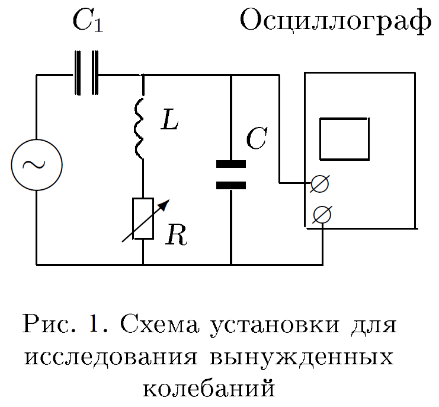
\includegraphics[width=1.99792in,height=1.85in]{./media/image1.png}


Для экспериментального исследования резонансной кривой тока в параллельном 
колебательном контуре используется схема, представленная на 
рис.~~\figref{forced oscillations scheme}. 
Синусоидальный сигнал с генератора подаётся на 
параллельный колебательный контур через небольшую разделительную 
ёмкость~$C_1$. 
Напряжение с конденсатора контура~$C$ поступает на вертикальный вход 
электронного осциллографа (ЭО). Для регистрации резонансной кривой необходимо,
чтобы модули импедансов возбуждающей~$Z_{ист}$ и измеряющей~$Z_{изм}$ 
цепей намного превосходили модуль импеданса самого контура вблизи 
резонанса $Z_{рез} \approx L/RC$.
\begin{wrapfigure}[13]{o}{0.45\linewidth}
    \pic{0.45\textwidth}{Chapter_2/2_5_2}
    \caption{Схема установки для исследования вынужденных колебаний}
    \figmark{forced oscillations scheme}
\end{wrapfigure}
С этой целью разделительная ёмкость~$C_1$ выбирается настолько малой, 
что в рабочем диапазоне частот модуль её импеданса $|Z_{C1}| = 1/\omega C_1$ 
много больше модуля импеданса контура на частоте $\omega$. 
Таким образом, амплитуда тока в цепи генератора определяется 
импедансом~$|Z_{C1}|$. Эта амплитуда относительно мало меняется 
в пределах резонансной кривой колебательного контура, что, однако, 
приводит к некоторому искажению последней по сравнению со случаем,
рассмотренным в п.~\ref{sec:ires}, где в качестве генератора
предполагается источник тока, обладающий большим 
и постоянным внутренним сопротивлением во всём исследуемом частотном диапазоне. 
Входное сопротивление осциллографа
(измеряющей цепи) достаточно велико: $|Z_{изм}|\approx R_{эо} \sim 1$~МОм, 
поэтому его влиянием можно пренебречь. 
Указанные ограничения представляются в виде следующих 
соотношений:
\begin{equation}
\eqmark{2.4.1}
|Z_{C_1}| = \frac{1}{\omega C_1} \gg \left| Z \right|_{рез} = \frac{Q}{\omega_0 C}, \qquad R_\text{эо} \gg \frac{Q}{\omega_0 C},
\end{equation}
где $Q \lesssim Q_m = \frac1R \sqrt{\frac{L}{C}}$ --- добротность контура, 
а $\omega_0$ --- его собственная циклическая частота. 

По полученной в эксперименте резонансной кривой $I_C(\omega)/I(\omega)$,
где $I_C$ --- ток через конденсатор в контуре, $I$ --- полный ток в цепи,
можно определить его резонансную частоту $\omega_m\approx \omega_0$ 
и добротность $Q$.
В~приближении, применимом для высокодобротного контура, 
$\omega_0$ будет совпадать с частотой максимума резонансной кривой, 
а добротность будет определяться 
её относительной шириной: $Q\approx \omega_0 / \delta \omega$
(см. \chaptereqref{2.63}).

Для установления более точной аналитической связи воспользуемся 
методом комплексных амплитуд. С~учётом условий~\eqref{2.4.1} 
исследуемая в работе схема эквивалентна рассмотренному в п.~\ref{sec:ires} 
случаю резонанса в \emph{параллельном} контуре. 
Вычислив модуль от первой формулы \chaptereqref{2.64}, можно получить 
следующее выражение
для резонансной кривой:
\begin{equation}
\eqmark{2.4.2}
\frac{I_C(\omega)}{I(\omega)} = 
%\frac{C U_C(\omega)}{C_1 U(\omega)} = 
%\frac{1+Q_0^2\left(\frac{\omega^2}{\omega_0^2}-1 \right)+iQ_0\frac{\omega_0}{\omega}}{%
%    1+Q_0^2\left(\frac{\omega}{\omega_0}-\frac{\omega_0}{\omega}\right)^2}
\sqrt{\frac{1+Q_m^2x^2}{1+Q_m^2(x-\frac1x)^2}},
\end{equation}
где $x=\omega/\omega_0$.

%$\vec U$  --- суммарное напряжение на ёмкости $C_1$ и колебательном контуре, 
%и .
Из соотношения \eqref{2.4.2} следует, 
что на \emph{собственной} частоте $\omega_0$ ток в \emph{высокодобротном} 
контуре почти в $Q\gg 1$ раз превосходит ток во внешней цепи. 
Именно по этой причине резонанс в параллельном контуре называется 
\emph{резонансом токов}. 
Отметим, что напряжение на контуре в принятом здесь приближении имеет ту 
же амплитудно-частотную характеристику, что и контурный ток:
\[
\frac{I_C(\omega)}{I(\omega)} = \frac{CU_C(\omega)}{C_1 U(\omega)},
\]
где $U$~--- суммарное напряжение на ёмкости $C_1$ и колебательном контуре.
При этом, как видно, отношение напряжений $U_C(\omega)/U(\omega)$ в $C/C_1\gg1$ 
раз меньше, чем отношение токов $I_C(\omega)/I(\omega)$.

Отметим также, что резонанс, то есть максимальный отклик на внешнее воздействие, 
достигается в данной схеме на частоте, несколько отличной от собственной частоты 
$\omega_0$, в чём можно убедиться при более детальном анализе формул \eqref{2.4.2}
(см. подробнее п.~\ref{sec:ires} Введения). 
Указанная особенность при не очень большой добротности контура легко регистрируется 
в эксперименте.


\labsection{Б. Процессы установления и затухания колебаний в контуре}

Добротность контура может быть определена и другими способами, например, 
по скорости нарастания амплитуды вынужденных колебаний при резонансе 
или по скорости затухания свободных колебаний. 

\begin{figure}[h!]
    \centering
    \pic{0.55\textwidth}{Chapter_2/2_5_3}
    \caption{Нарастание и затухание вынужденных колебаний}
    \figmark{forced oscillations damping}
\end{figure}

Нарастание и затухание 
колебаний (рис.~\figref{forced oscillations damping}) можно наблюдать 
на экране осциллографа, если на контур подаются \emph{цуги} --- отрезки 
синусоиды, разделённые интервалами, в течение которых сигнал отсутствует. 
Чем выше добротность~$Q$, тем медленнее 
нарастают и медленнее затухают колебания в контуре. Получить значение $Q$ 
можно, измерив логарифмический декремент затухания по скорости 
нарастания или затухания колебаний. В~условиях резонанса огибающая затухающих 
колебаний --- это <<перевёрнутая>> огибающая нарастающего участка 
(см. формулу \chaptereqref{2.73}).
Она может быть использована для расчёта логарифмического декремента затухания
по формуле \chaptereqref{2.75}.
%При этом нет необходимости использовать амплитуду установившихся 
%колебаний~$U_0$, которая в контуре с высокой добротностью может не успеть 
%установиться за время продолжительности цуга.



\experiment 


Схема установки для исследования вынужденных колебаний приведена 
на рис.~\figref{forced oscillations exp scheme}. 
Колебательный контур 
состоит из конденсатора с ёмкостью~$C$, катушки с индуктивностью~$L$ и 
магазина сопротивлений~$R$. 
Сигнал, состоящий из отрезков синусоиды (цуги), может генерироваться
либо цифровым генератором электрических сигналов произвольной формы,
либо комбинацией генератора синусоиадльного сигнала звукового 
диапазона (ЗГ) и электронного реле, прерывающего сигнал с заданной периодичностью. 
Результирующий сигнал 
поступает через небольшую ёмкость~$C_1$ на клеммы, 
смонтированные на отдельной панели. 
Жирной линией отмечен кабель, содержащий 4 изолированных проводника, 
идущие от генераторов к двум конденсаторам~$C_1$, 
разъёмам <<синхр.>> (синхронизация) и <<$\bot$>> (земля). При подключении 
контура к клеммам~<<$\perp$>> и~<<непр.>> на него подаётся непрерывный 
сигнал~--- синусоида; если контур подключён к клеммам~<<$\perp$>> и~<<цуги>>~--- 
на контур поступают отрезки синусоиды.


\begin{figure}[h]
    \centering
\small	\pic{0.9\textwidth}{Chapter_2/2_5_4}
	\caption{Схема экспериментальной установки для исследования вынужденных
колебаний}
	\figmark{forced oscillations exp scheme}
\end{figure}

Для визуального наблюдения за процессом колебаний напряжение с ёмкости 
контура~$C$ подаётся на вход электронного осциллографа. Чтобы картина на 
экране была устойчивой, частота развёртки осциллографа принудительно 
синхронизуется с частотой повторения цугов. Для этого на генератор 
развёртки ЭО подаются следующие с частотой повторения цугов управляющие 
импульсы, формируемые в блоке электронного реле, клемма <<синхр.>> которого 
смонтирована на отдельной панели. Для измерений напряжения на ёмкости~$C$ 
используется цифровой вольтметр~$V$.

Используя представленную схему в режиме непрерывного синусоидального 
сигнала, можно по показаниям приборов и известных параметров элементов 
цепи измерить амплитудную характеристику (резонансную кривую) 
$I_C(\omega)/I(\omega)$ в необходимом диапазоне частот. 
Сравнивая результат измерения с теоретической кривой \eqref{2.4.2}, можно 
определить характеристики колебательного контура $\omega_0$ и $Q$.
 
\begin{lab:task}

\taskpreamble{%
     В работе предлагается исследовать резонансные кривые при подаче 
     на колебательный контур непрерывного гармонического сигнала и определить 
     по ним резонансную частоту и добротность контура при двух значениях 
     его активного сопротивления; затем определить добротность, измерив 
     логарифмический декремент затухания при нарастании и при затухании 
     колебаний в режиме генерации цугов.}
    
\tasksection{I. Подготовка приборов к работе}

	\item Соберите схему согласно рис.~\figref{forced oscillations exp scheme}
	и подключите контур к клеммам «$\perp$» и <<непр.>>. Включите приборы в сеть. 
    Руководствуясь техническим описанием установки, настройте генератор, 
    осциллограф, проверьте работоспособность источника питания, 
    а также установите необходимые значения на магазинах сопротивлений 
    и индуктивностей.

\tasksection{II. Исследование резонансных кривых}

	\item Рассчитайте собственную частоту контура $\nu_{0} = 1/2\pi\sqrt{LC}$.

	\item Изменяя частоту генератора вблизи собственной и наблюдая за синусоидой 
    на экране осциллографа, убедитесь, что в резонансе, когда амплитуда колебаний 
    максимальна, частота колебаний близка к собственной частоте контура. 
    Подберите частоту развёртки осциллографа и амплитуду синхронизации, 
    при которых картина неподвижна.

	\item Меняя частоту генератора в обе стороны от резонансной, получите зависимость 
    показаний вольтметра~$U$ от частоты сигнала~$\nu$. 
    Расчёт добротности ведётся на уровне $\sim 0,707$ от резонансной амплитуды, 
    поэтому стоит аккуратнее провести измерения в районе этого уровня, 
    а также продолжать измерения, по крайней мере, до тех пор, пока амплитуда 
    сигнала упадёт до величины 0,3--0,4 от резонансной.

	\item Установите на магазине сопротивлений другое значение, заданное
преподавателем, и повторите измерения предыдущего пункта. 
%Закончив измерения, отключите вольтметр от сети.

\tasksection{III. Процессы установления и затухания колебаний}

	\item Подключите контур к клеммам <<цуги>> и <<$\perp$>>. 
    Установите нулевое сопротивление магазина.

	\item Установите на генераторе собственную частоту контура. Подберите частоту 
    развёртки осциллографа, при которой на экране умещается один цуг колебаний. 
    Убедитесь, что огибающая затухающих колебаний~--- это перевёрнутая огибающая 
    нарастающего участка. Если они заметно отличаются (реле может внести искажения), 
    то следует уменьшить амплитуду сигнала, поступающего от генератора.

	\item \label{p-damp} Для расчёта добротности по скорости нарастания амплитуды измерьте
амплитуды двух колебаний $U_k$ и $U_{k+n}$, разделённых целым числом периодов $n$,
и амплитуду установившихся колебаний $U_{\infty}$ 
(см. рис.~\figref{forced oscillations damping}).

Перед началом измерений заземлите канал $Y$, чтобы уточнить положение 
горизонтальной оси~--- начала отсчёта амплитуды. 
Следует увеличить амплитуду, сместив горизонтальную ось симметрии цуга в нижнюю часть 
экрана. Расчёт будет тем точнее, чем больше отличаются друг от друга все 
три амплитуды.

Проведите измерения для 4--5 пар амплитуд.

	\item \label{p-raise} Для определения добротности по скорости затухания измерьте две
амплитуды, разделённые целым числом периодов (для 4--5 пар амплитуд).

	\item Повторите измерения п.~\ref{p-damp}, \ref{p-raise} для другого 
    значения сопротивления, заданного преподавателем.

	\item Сместите частоту генератора от резонансного значения и получите на
экране картину биений. Зарисуйте и объясните эту картину.

	\item Отключите приборы от сети и разберите схему.

	\item Измерьте активное сопротивление~$R_L$ и индуктивность~$L$ магазина
индуктивностей с помощью измерителя импедансов ($LCR$-метра) 
на частотах $50$~Гц, $500$~Гц и $1500$~Гц. По указанию преподавателя 
используйте $LCR$-метр для измерения других параметров установки.

\tasksection{IV. Обработка результатов}

	\item Постройте на одном графике резонансные кривые для использованных значений
    сопротивления $R$ в координатах $U/U_0 = f(\nu/\nu_0)$, 
    где $U_0$~---~напряжение при резонансной частоте $\nu_0$.
    Сравните резонансные кривые и определите сопротивление катушки индуктивности
    $R_L$.
    \item Определите добротность по формуле $Q \approx \nu_0/(2\delta\nu)$,
    где $2\delta \nu$ --- ширина резонансной кривой на уровне $0,707$.
    Сравните теоретическое и экспериментальное значения резонансной частоты.

	\item Рассчитайте добротность контура по скорости нарастания и затухания
колебаний.

	\item Рассчитайте теоретическое значение добротности через параметры
контура $L$, $C$ и $R$.

\item Сведите результаты определения $Q$ в таблицу, где $R_{\Sigma}=R_L+R$:
\begin{center}\small
\begin{tabular}{|c|c|c|c|c|c|}
\hline
& & \multicolumn{4}{c|}{$Q$}\\
\cline{3-6}
$R$, Ом & $R_{\Sigma}$ & 
\parbox{2cm}{Ширина\\[-4pt] рез. кривой} & Нарастание & Затухание &$f(LCR)$\\
\hline
$0$ & & & & & \\
$100$ & & & & &\\
\hline
\end{tabular}
\end{center}
%
%\begin{figure}[h!]
%	\centering
%	%\pic{0.6\linewidth}{Chapter_2/image4}
%	\caption{Таблица}
%\end{figure}
%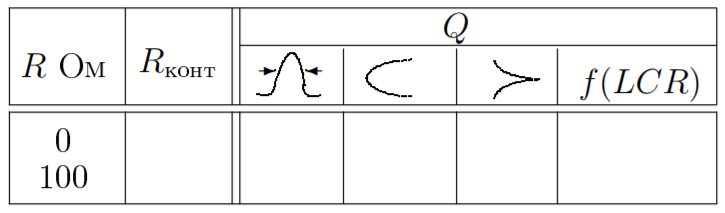
\includegraphics[width=3.37592in,height=0.99167in]{./media/image4.png}
	\item Оцените погрешности, сравните результаты расчётов. Объясните
    различие результатов, полученных разными методами.
\end{lab:task}


\begin{lab:questions}
    \item Опишите известные вам способы измерения добротности колебательного контура.
    \item Дайте энергетическое определение добротности колебательной системы.
    \item Что называется импедансом электрической цепи?
        Как складываются импедансы при последовательном и параллельном
        соединении элементов электрической цепи?
    \item С каким «запасом» выполняются условия \eqref{2.4.1} в данной работе?
    \item Выведите формулу \eqref{2.4.2}.
\end{lab:questions}


\begin{lab:literature}
	\item \SivuhinIII~--- \S~122--124.

	\item \Kalashnikov~--- \S~207--210.
\end{lab:literature}
